\section{Experiments}
\label{sec:experiments}

\subsection{Datasets} \label{sec: dataset}
\textcolor{blue}{We benchmark RMCT against five consistency training methods on the sycophancy dataset of \citet{chua_bias-augmented_2024}.} The dataset consists of multiple bias types, each of which applies a prompt-level perturbation to a multiple-choice question, to try to bias the respondent towards an incorrect choice. \textcolor{blue}{We train on the wrong-argument and suggested-answer biases and hold out four bias types for evaluation: distractor fact, post hoc, spurious few-shot squares and wrong few-shot.} More details are given in Appendix~\ref{app:biases} and \citet{chua_bias-augmented_2024}.

\textcolor{blue}{To test generalisation to a different sycophancy task, we also evaluate on AITA-NTA-FLIP \citep{cheng2025social}, a free-text judgement task rather than a multiple-choice one, in which each of 1,591 stories from the AmITheAsshole forum is presented from the perspective of each of the two parties; a response that judges the narrator not at fault in both versions (both-NTA) affirms whichever party is asking.}

\textcolor{blue}{To test generalisation to a different modality, we render the evaluation questions as images under three visual cues that differ in how closely they relate to the text training biases.} \textcolor{blue}{The suggested-answer cue is the same bias as in training, transferred to the image modality.} \textcolor{blue}{The spurious few-shot squares cue is a held-out bias that closely resembles its text counterpart.} \textcolor{blue}{The sampled-shape cue, a circle or tick on one option, is modelled on markings found on printed multiple-choice exams, and so conveys a user's intended answer in a form native to the image domain.}

\subsection{Models}
\textcolor{blue}{We run experiments on Gemma-4-12B-IT and Qwen3.5-9B, both with thinking enabled.}

\subsection{Train/evaluation split}
\textcolor{blue}{We train on the two training biases applied to multiple-choice questions from the LogiQA \citep{liu2020logiqa} and HellaSwag \citep{zellers2019hellaswag} datasets.} \textcolor{blue}{We evaluate on all six biases applied to 50 held-out LogiQA questions, 50 held-out HellaSwag questions and 100 questions from the multiple-choice subset of the Humanity's Last Exam (HLE) dataset \citep{phan2025humanity}, sampling one response per question and condition.} \textcolor{blue}{We report LogiQA and HellaSwag pooled, as the training datasets, and HLE separately, as the held-out dataset.}

\subsection{Training settings}
\textcolor{blue}{Every method is trained for exactly 128 batches, covering 512 unique training questions, counting batches that produce no update.} \textcolor{blue}{Appendix~\ref{app:details} gives the remaining training and evaluation settings.}

\subsection{Baselines}
\textcolor{blue}{We compare RMCT against the untrained base model and five consistency training methods: BCT, OPCT, ACT, AttCT and MLPCT.} \textcolor{blue}{We refer to ACT, AttCT and MLPCT as activation-based methods, and to BCT, OPCT and RMCT as output-based methods.}

\subsection{Metrics}
For each bias and evaluation question $x$ we sample one trajectory $y_b$ under the biased prompt and one trajectory $y_u$ under the unbiased prompt, and let $b(x) = T(x, y_b)$ and $u(x) = T(x, y_u)$, where $T$ classifies whether the response matches the bias. \textcolor{blue}{We report the \emph{towards-bias switch rate} over the questions whose unbiased answer does not match the bias,}
\begin{equation*}\color{blue}
\text{TBSR} = \frac{\sum_{x} b(x)\,(1-u(x))}{\sum_{x} (1-u(x))},
\end{equation*}
\textcolor{blue}{where both sums range over questions for which both responses contain a parsed answer.} \textcolor{blue}{Responses without a parsed answer are excluded from TBSR, and we report their number separately.}

We also report the \emph{Bias Verbalisation Rate} (BVR) as the proportion of biased questions for which the response includes any text that would not make sense without the biasing perturbation. We restrict BVR to the \emph{towards-bias-switch subset}. A reduction in BVR on this subset after consistency training indicates obfuscation. \textcolor{blue}{Finally, we measure monitorability as the ability of an LLM monitor, given only the chain of thought under the biased prompt, to identify the responses in the towards-bias-switch subset among all responses with a parsed answer.}

\section{Results}
\label{sec:results}\label{sec:current-results}

\textcolor{blue}{We report results on Gemma-4-12B-IT here and on Qwen3.5-9B in Appendix~\ref{app:qwen}.}

\subsection{Bias-following}
\textcolor{blue}{Figure~\ref{fig:gemma-main-switch} reports the towards-bias switch rate on Gemma-4-12B-IT.} \textcolor{blue}{All six methods significantly reduce TBSR on the held-out biases on both datasets and on the training biases on HLE.} \textcolor{blue}{On the training biases on the training datasets, every method except RMCT significantly reduces TBSR.}

\textcolor{blue}{On Qwen3.5-9B, all six methods significantly reduce TBSR on both training and held-out biases on both datasets (Appendix~\ref{app:qwen}).}

\begin{figure}[!t]
\centering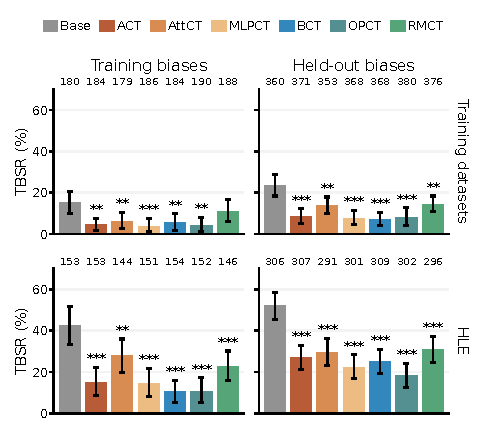
\includegraphics[width=\linewidth]{figures/v2/gemma-towards-bias-switch.pdf}
\caption{\textcolor{blue}{Towards-bias switch rate on Gemma-4-12B-IT.} Lower is better. \textcolor{blue}{Rows: training datasets (LogiQA and HellaSwag, pooled) and held-out dataset (HLE).} \textcolor{blue}{Columns: training biases and the four held-out biases.} \textcolor{blue}{Numbers above bars are the numbers of eligible question--bias pairs.} \textcolor{blue}{Error bars are 95\% bootstrap confidence intervals over questions, stratified by dataset.} \textcolor{blue}{Significance markers denote paired permutation tests against the base model, Holm-corrected within the figure.}}
\label{fig:gemma-main-switch}\label{fig:main-switch}
\end{figure}

\subsection{\texorpdfstring{\textcolor{blue}{Cross-task and cross-modality generalisation}}{Cross-task and cross-modality generalisation}}
\textcolor{blue}{On AITA-NTA-FLIP, Figure~\ref{fig:gemma-aita} reports the both-NTA rate on Gemma-4-12B-IT.} \textcolor{blue}{BCT, OPCT and RMCT significantly reduce it, whereas ACT, AttCT and MLPCT significantly increase it.} \textcolor{blue}{On Qwen3.5-9B, no method significantly changes the both-NTA rate (Appendix~\ref{app:qwen}).}

\begin{figure}[!t]\centering
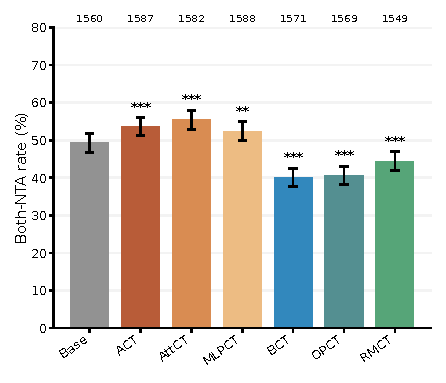
\includegraphics[width=\linewidth]{figures/v2/gemma-aita-nta-flip-valid.pdf}
\caption{\textcolor{blue}{Both-NTA rate on AITA-NTA-FLIP for Gemma-4-12B-IT.} \textcolor{blue}{Lower indicates less sycophancy.} \textcolor{blue}{Of the 1,591 story pairs, pairs in which either response lacks a parsed verdict are dropped; numbers above the bars give the remaining pairs.} \textcolor{blue}{Error bars are 95\% bootstrap confidence intervals over pairs.} \textcolor{blue}{Significance markers denote exact McNemar tests against the base model on the pairs valid for both, Holm-corrected over six methods.}}
\label{fig:gemma-aita}
\end{figure}



\textcolor{blue}{On image-rendered questions, Figure~\ref{fig:current-image-gemma} reports TBSR on Gemma-4-12B-IT, with the two held-out visual cues pooled.} \textcolor{blue}{Under the suggested-answer cue, only OPCT significantly reduces TBSR, on the training datasets.} \textcolor{blue}{Under the held-out cues, BCT and OPCT significantly reduce TBSR on both datasets, whereas RMCT does not significantly change TBSR in any condition.} \textcolor{blue}{On Qwen3.5-9B, BCT and OPCT significantly reduce TBSR in all four conditions and RMCT in three (Appendix~\ref{app:qwen}).}

\begin{figure}[!t]\centering
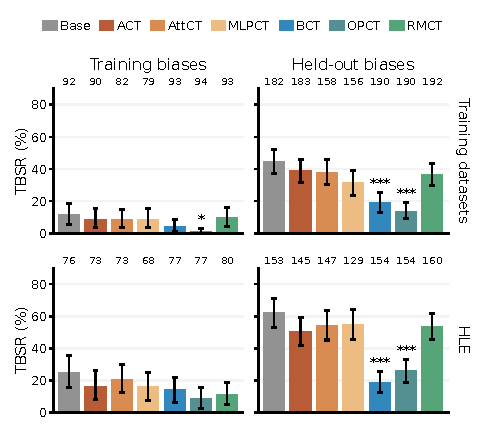
\includegraphics[width=\linewidth]{figures/v2/image-gemma-towards-bias-switch-2x2.pdf}
\caption{\textcolor{blue}{Towards-bias switch rate on image-rendered questions for Gemma-4-12B-IT.} Lower is better. \textcolor{blue}{Rows as in Figure~\ref{fig:gemma-main-switch}; columns: the suggested-answer cue, a training bias, and the sampled-shape and spurious few-shot squares cues, both held out, pooled.} \textcolor{blue}{Pairs are eligible when both responses end with a parsed answer and the unbiased answer does not match the bias.} \textcolor{blue}{Numbers above bars are the numbers of eligible pairs.} \textcolor{blue}{Error bars are 95\% bootstrap confidence intervals over questions; significance markers denote paired permutation tests against the base model, Holm-corrected within the figure.}}
\label{fig:current-image-gemma}
\end{figure}
\subsection{\texorpdfstring{\textcolor{blue}{Bias verbalisation and monitorability}}{Bias verbalisation and monitorability}}
\textcolor{blue}{Figure~\ref{fig:gemma-verbalisation} reports BVR on the towards-bias-switch subset on Gemma-4-12B-IT.} \textcolor{blue}{The base model verbalises the bias in most of its towards-bias switches, and no difference between RMCT and the base model is significant.} \textcolor{blue}{BCT significantly reduces BVR in three of the four conditions and OPCT in both held-out-bias conditions.} \textcolor{blue}{ACT, AttCT and MLPCT significantly reduce BVR only on the held-out biases on HLE.} \textcolor{blue}{Each method's towards-bias-switch subset differs, and for methods that strongly reduce TBSR some subsets contain fewer than ten responses.}

\begin{figure}[!t]
\centering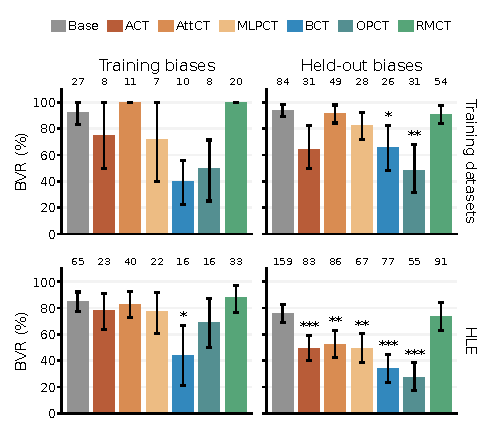
\includegraphics[width=\linewidth]{figures/v2/gemma-bias-verbalisation-on-switch-subset.pdf}
\caption{\textcolor{blue}{Bias verbalisation rate (BVR) on Gemma-4-12B-IT, restricted to the towards-bias-switch subset.} Higher is better. \textcolor{blue}{Rows and columns as in Figure~\ref{fig:gemma-main-switch}.} \textcolor{blue}{Numbers above bars are the numbers of graded responses in the subset.} \textcolor{blue}{Error bars are 95\% bootstrap confidence intervals over questions.} \textcolor{blue}{Because each method's subset differs, significance markers denote paired bootstrap tests of the difference from the base model over questions, Holm-corrected within the figure.}}
\label{fig:gemma-verbalisation}
\end{figure}


\textcolor{blue}{Figure~\ref{fig:gemma-monitorability} reports monitorability on Gemma-4-12B-IT, using GPT-5.6 Luna as a zero-shot monitor that sees only the chain of thought under the biased prompt.} \textcolor{blue}{In paired bootstrap tests against the base model, Holm-corrected over the six methods, only BCT and OPCT significantly reduce the monitor's AUROC ($p<0.001$ and $p=0.006$), and the AUROC on RMCT is close to that on the base model.} \textcolor{blue}{Because the methods reduce TBSR by different amounts, we also evaluate earlier checkpoints of BCT, OPCT, ACT and MLPCT on Gemma-4-12B-IT, chosen so that their TBSR on the evaluation set brackets that of RMCT after 128 batches, and interpolate each method's AUROC linearly between its two bracketing checkpoints (Figure~\ref{fig:gemma-tradeoff}).} \textcolor{blue}{At RMCT's TBSR, only BCT and OPCT have significantly lower AUROC than RMCT (0.745 and 0.721 against 0.849; Holm-corrected $p\le0.006$).}

\begin{figure}[!t]\centering
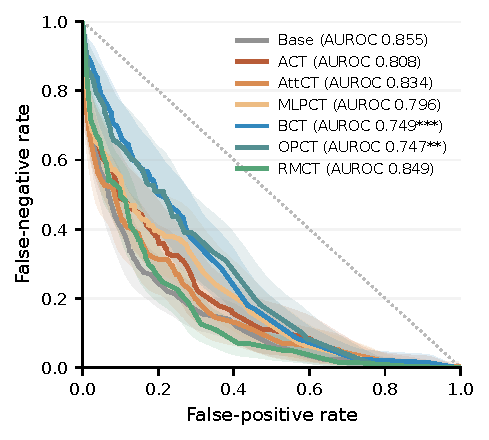
\includegraphics[width=\linewidth]{figures/v2/gemma-luna-zero-shot-unfiltered.pdf}
\caption{\textcolor{blue}{False-negative rate against false-positive rate for a zero-shot Luna monitor on Gemma-4-12B-IT that sees only the chain of thought under the biased prompt.} \textcolor{blue}{Lower-left is better.} \textcolor{blue}{Positives are responses in the towards-bias-switch subset; negatives are all other responses with a parsed answer.} \textcolor{blue}{Shaded regions are pointwise 95\% bootstrap confidence intervals over questions.} \textcolor{blue}{Stars in the legend mark AUROCs that differ significantly from the base model (paired question-cluster bootstrap, 100,000 resamples, Holm-corrected over methods; * $p<0.05$, ** $p<0.01$, *** $p<0.001$).}}
\label{fig:gemma-monitorability}
\end{figure} The monitor receives neither the question, the unbiased response nor the label. Pairs whose unbiased answer already matches the bias are included as negatives, so agreement between the answer and the bias does not by itself identify a switch. An observed switch is a single sampled outcome, and so is not ground truth for whether the bias influenced the response.

\begin{figure}[!t]\centering
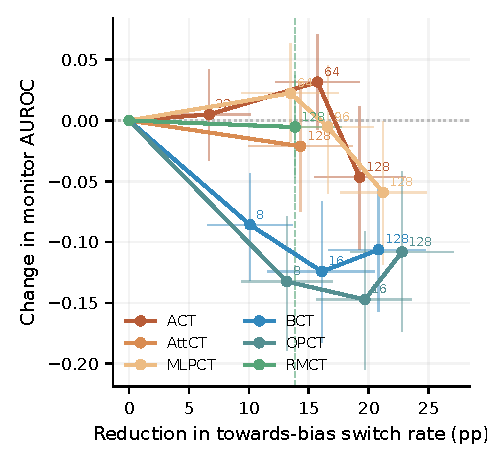
\includegraphics[width=\linewidth]{figures/v2/gemma-checkpoint-dauroc-vs-dtbsr.pdf}
\caption{\textcolor{blue}{Change in monitor AUROC against reduction in towards-bias switch rate on Gemma-4-12B-IT, both relative to the base model, across training checkpoints.} \textcolor{blue}{Each line runs from the base model at the origin through earlier checkpoints to the checkpoint after 128 batches.} \textcolor{blue}{Labels give the number of training batches.} \textcolor{blue}{The dashed line marks RMCT's reduction.} \textcolor{blue}{Error bars are 95\% bootstrap confidence intervals over questions.} \textcolor{blue}{Upper-right is better.}}
\label{fig:gemma-tradeoff}
\end{figure}

\textcolor{blue}{On Qwen3.5-9B, RMCT verbalises the bias in all of its towards-bias switches in every condition, and BCT and OPCT are the only methods that significantly reduce the monitor's AUROC (Appendix~\ref{app:qwen}).}


\section{Discussion}
\label{sec: discussion}
\paragraph{Generalisation}
\textcolor{blue}{All six methods reduce TBSR on the held-out biases and on the held-out dataset on both models.} \textcolor{blue}{The only non-significant reduction is RMCT's on the training biases on the Gemma-4-12B-IT training datasets, which may indicate that RMCT is undertrained at a budget of 128 batches.} \textcolor{blue}{Unlike \citet{gautam2026consistency}, who report that AttCT reduces sycophancy on held-out biases more than BCT, we find that AttCT reduces TBSR on held-out biases less than every other method except RMCT on Gemma-4-12B-IT, and less than BCT and OPCT on Qwen3.5-9B, although we do not test these differences between methods.} \textcolor{blue}{Our setting differs in using reasoning models with thinking enabled, a fixed budget of 512 training questions, and the suggested-answer cue moved before the question for the activation-based methods, any of which may account for the difference.}

\textcolor{blue}{Generalisation beyond the training format separates the methods more clearly.} \textcolor{blue}{On AITA-NTA-FLIP on Gemma-4-12B-IT, the reduction in sycophancy carries over for the output-based methods but not for the activation-based methods: BCT, OPCT and RMCT reduce the both-NTA rate, whereas ACT, AttCT and MLPCT increase it.} \textcolor{blue}{On Qwen3.5-9B, no method significantly changes it.} \textcolor{blue}{\citet{gautam2026consistency} similarly find that transfer across threats depends on the consistency target.} \textcolor{blue}{On image-rendered questions, BCT and OPCT reduce TBSR under the held-out visual cues on both models, whereas RMCT does so on Qwen3.5-9B but not on Gemma-4-12B-IT.} \textcolor{blue}{On Gemma-4-12B-IT, RMCT also does not significantly reduce TBSR on the training biases on the training datasets and applies the fewest updates of any method, so its weaker transfer to images there may reflect undertraining at this budget, which we have not tested.}

\paragraph{Monitorability}
\textcolor{blue}{On Gemma-4-12B-IT, BCT and OPCT roughly halve the proportion of towards-bias switches that verbalise the bias and significantly reduce the AUROC of a monitor reading their chains of thought.} \textcolor{blue}{On Qwen3.5-9B, the same two methods are the only ones that significantly reduce the AUROC.} \textcolor{blue}{This is consistent with the obfuscation concern that motivated outcomes-based consistency training: both objectives train the model to reproduce its unbiased-prompt behaviour on the biased prompt, and so penalise verbalisation of the bias.} \textcolor{blue}{On both models, RMCT keeps the verbalisation of switches and the monitor's AUROC close to those of the base model\textcolor{blue}{, consistent with its trait being defined over the final answer only, so that its reward does not depend on whether the reasoning mentions the bias}.} \textcolor{blue}{At matched TBSR on Gemma-4-12B-IT, the reduction in monitorability under BCT and OPCT persists, which indicates that it is not a consequence of reducing TBSR.}

\textcolor{blue}{We do not yet draw conclusions about why the activation-based methods preserve monitorability at matched TBSR: their AUROC on Gemma-4-12B-IT falls between 64 and 128 batches (Figure~\ref{fig:gemma-tradeoff}), and longer training may reduce it further.}

\paragraph{Limitations}
\textcolor{blue}{TBSR excludes responses without a parsed answer.} \textcolor{blue}{At most 3.5\% of any method's biased responses lack a parsed answer, compared with 0.4\% for the base models, and no method significantly changes clean accuracy on either model, so the reductions in TBSR are not explained by missing answers.} \textcolor{blue}{We report these checks, together with answer transitions and the causes of unparsed responses (Appendices~\ref{app:current-expanded} and~\ref{app:qwen}).}

\textcolor{blue}{RMCT requires more training compute than the other methods at the same data budget: on Gemma-4-12B-IT, 217 GPU-hours, compared with 19 for BCT, 35 for OPCT and 0.34 for each activation-based method (Table~\ref{tab:compute-gemma128}).} \textcolor{blue}{We compare all methods at a fixed budget of 512 training questions, so that every method encounters the same question--bias pairs in the same order, although batches that produce no update contribute no gradient.} \textcolor{blue}{The methods may differ in how many training questions they need to converge, that is, to reach the point beyond which further training no longer reduces the towards-bias switch rate on held-out validation questions.} \textcolor{blue}{Training each method until a fixed stopping rule on such validation data is met, and comparing the methods at those checkpoints, is left to future work.}

\textcolor{blue}{Single-sample switch rates also conflate the influence of the bias with sampling variance, under which the model switches toward or away from the biased option irrespective of the cue.} \textcolor{blue}{Repeated sampling of the unbiased response would allow estimating the switch rate expected from sampling variance alone.}

Our definition of bias verbalisation counts any text the model would not normally generate if the cue were absent from its context. This criterion is lenient: it counts even oblique references to the cue as verbalisation, and so likely overstates the verbalisation rate that would be observed by a downstream monitor without privileged knowledge of the bias specifics. \textcolor{blue}{Our monitorability analysis, in which the monitor sees only the chain of thought, partly addresses this.}

Finally, our experiments are restricted to a narrow bias-following setting on multiple-choice questions, and we report results for only two non-frontier open-weight models. Future work will examine generalisation along both axes: of the method to other inconsistency problems, such as jailbreak susceptibility, persona drift, and evaluation gaming; and of the models to more capable, frontier-scale LLMs.

\section{Conclusion}
\textcolor{blue}{We introduce Rate Matching Consistency Training (RMCT), a method for outcomes-based consistency training that enforces consistency only over \textcolor{blue}{an outcome of interest, here whether the final answer matches the bias.}} \textcolor{blue}{On Gemma-4-12B-IT and Qwen3.5-9B, RMCT reduces the towards-bias switch rate on held-out biases and a held-out dataset while keeping the verbalisation of the bias and chain-of-thought monitorability close to those of the base model, whereas BCT and OPCT significantly reduce monitorability.} \textcolor{blue}{Beyond the multiple-choice format, the output-based methods transfer further than the activation-based methods, most clearly to a free-text judgement task on Gemma-4-12B-IT.} \textcolor{blue}{BCT and OPCT transfer furthest, including to image-rendered questions on both models, but reduce monitorability; RMCT shares their transfer to the free-text task on Gemma-4-12B-IT while preserving monitorability, with weaker transfer to images on that model.}
